\documentclass[10pt,t]{beamer}


\setbeamersize{text margin left=10pt,text margin right=10pt}
\usetheme{lehigh}

\usefonttheme{professionalfonts}
\usefonttheme{serif}

% add packages to use
\usepackage{tabularx}
\usepackage{tikz}
\usetikzlibrary{trees,matrix,shapes,arrows}
\usetikzlibrary{calc}
\usepackage{fancyvrb}
\usepackage{listings}

\pgfdeclarelayer{background}
\pgfdeclarelayer{foreground}
\pgfsetlayers{background,main,foreground}
\usepackage[latin1]{inputenc}
\usepackage[english]{babel}
\usepackage{hyperref}
\usepackage[normalem]{ulem}

                                                         
%\usepackage{times}
%\usepackage[T1]{fontenc}
\usepackage{graphicx}
%\usepackage{pgf,pgfarrows,pgfnodes,pgfautomata,pgfheaps,pgfshade}
\usepackage{amsmath,amssymb,amsfonts,subfigure,pifont}
\usepackage{multirow}
\usepackage{booktabs}
\usepackage{colortbl}
\usepackage{keystroke}
\usepackage{etex}


% The following color are for listing environment 
\definecolor{dkgreen}{rgb}{0,0.6,0}
%\definecolor{gray}{rgb}{0.5,0.5,0.5}
\definecolor{mauve}{rgb}{0.58,0,0.82}


\lstset{%
language=bash,                % the language of the code
basicstyle=\tiny\ttfamily,           % the size of the fonts that are used for the code
showspaces=false,               % show spaces adding particular underscores
showstringspaces=false,         % underline spaces within strings
showtabs=false,                 % show tabs within strings adding particular underscores
%frame=single,                   % adds a frame around the code
%rulecolor=\color{black},        % if not set, the frame-color may be changed on line-breaks within not-black text (e.g. comments (green here))
tabsize=2,                      % sets default tabsize to 2 spaces
%captionpos=b,                   % sets the caption-position to bottom
breaklines=true,                % sets automatic line breaking
breakatwhitespace=false,        % sets if automatic breaks should only happen at whitespace
%title=\lstname,                   % show the filename of files included with \lstinputlisting;
% also try caption instead of title
keywordstyle=\color{blue},          % keyword style
commentstyle=\color{dkgreen},       % comment style
stringstyle=\color{mauve},         % string literal style
escapeinside={!}{!},            % if you want to add LaTeX within your code
morekeywords={*,\dots,elif},              % if you want to add more keywords to the set
deletekeywords={\dots},              % if you want to delete keywords from the given language
%morecomment=[l]{//}
}
\lstset{%
language=csh,                % the language of the code
basicstyle=\tiny\ttfamily,           % the size of the fonts that are used for the code
showspaces=false,               % show spaces adding particular underscores
showstringspaces=false,         % underline spaces within strings
showtabs=false,                 % show tabs within strings adding particular underscores
%frame=single,                   % adds a frame around the code
%rulecolor=\color{black},        % if not set, the frame-color may be changed on line-breaks within not-black text (e.g. comments (green here))
tabsize=2,                      % sets default tabsize to 2 spaces
captionpos=b,                   % sets the caption-position to bottom
breaklines=true,                % sets automatic line breaking
breakatwhitespace=false,        % sets if automatic breaks should only happen at whitespace
%title=\lstname,                   % show the filename of files included with \lstinputlisting;
% also try caption instead of title
keywordstyle=\color{blue},          % keyword style
commentstyle=\color{dkgreen},       % comment style
stringstyle=\color{mauve},         % string literal style
escapeinside={\%*}{*)},            % if you want to add LaTeX within your code
morekeywords={*,\dots,elif},              % if you want to add more keywords to the set
deletekeywords={\dots},              % if you want to delete keywords from the given language
%morecomment=[l]{//}
}

\lstdefinestyle{LINUX}
{
    backgroundcolor=\color{white},
    basicstyle=\tiny\ttfamily,
    keywordstyle=\color{blue},
    morekeywords={apacheco,Tutorials,BASH,scripts,day1,examples},
    literate={>}{{\textcolor{blue}{>}}}1
         {/}{{\textcolor{blue}{/}}}1
         {./}{{\textcolor{black}{./ }}}1
         {~}{{\textcolor{blue}{\textasciitilde}}}1,
}



\DeclareSymbolFont{extraup}{U}{zavm}{m}{n}
%\DeclareMathSymbol{\vardiamond}{\mathalpha}{extraup}{87}
\newcommand{\cmark}{\ding{51}}
\newcommand{\xmark}{\ding{55}}
\newcommand{\smark}{\ding{77}}
\newcommand*\vardiamond{\textcolor{lubrown}{%
  \ensuremath{\blacklozenge}}}
\newcommand*\mybigstar{\textcolor{lubrown!90!yellow}{%
  \ensuremath{\bigstar}}}
\newcommand*\up{\textcolor{green!80!black}{%
  \ensuremath{\blacktriangle}}}
\newcommand*\down{\textcolor{red}{%
  \ensuremath{\blacktriangledown}}}
\newcommand*\const{\textcolor{darkgray}%
  {\textbf{--}}}
\newcommand*\enter{\tikz[baseline=-0.5ex] \draw[<-] (0,0) -| (0.5,0.1);}

\newcommand{\Verblubrown}[1]{\Verb[formatcom=\color{lubrown},fontseries=b,commandchars=\\\{\}]|#1|}
\newcommand{\Verblue}[1]{\Verb[formatcom=\color{lublue},fontseries=b,commandchars=\\\{\}]!#1!}
\newcommand{\Verbblue}[2][b]{\Verb[formatcom=\color{lublue},fontshape=#1,commandchars=\\\{\}]|#2|}
\newcommand{\Verblubrownp}[1]{\Verb[formatcom=\color{lubrown},fontseries=b,commandchars=\\\{\}]!#1!}


% LOGOS
% footer logo
\pgfdeclareimage[width=0.3\paperwidth]{university-logo}{lulogo}
\tllogo{\pgfuseimage{university-logo}}

%titlepage logo
\titlegraphic{\includegraphics[scale=0.5]{lu}}


\beamertemplateballitem
\usetikzlibrary{mindmap,trees}
\usetikzlibrary{decorations.text,calc,arrows.meta}

\definecolor{luorange}{RGB}{255,196,35}
\definecolor{luorange2}{RGB}{255,226,147}

%% Tikz Distro Watch Table
% Defining some symbols:
\newcommand*\head[1]{\textbf{#1}}
% The table environment:
\newenvironment{matrixtable}[4]{%
  \begin{tikzpicture}[matrix of nodes/.style={
    execute at begin cell=\node\bgroup\strut,
    execute at end cell=\egroup;}]
  \matrix (m) [matrix of nodes,top color=blue!20,
    bottom color=blue!80,draw=white,
    nodes={draw,top color=blue!10,bottom color=blue!35,
    draw,inner sep=2pt,minimum height=3.1ex},
    column sep=1ex,row sep=0.6ex,inner sep=2ex,
    rounded corners,column 1/.style={minimum width=#1},
    column 2/.style={minimum width=#2},
    column 3/.style={minimum width=#3},
    column 4/.style={minimum width=#4}]}%
{;\end{tikzpicture}}

\title{Introduction to Linux}
\subtitle{Basic Commands \& Environment}
\author{Alexander B. Pacheco}
\institute{\href{http://researchcomputing.lehigh.edu}{LTS Research Computing}}%\\[2pt] \href{http://www.lehigh.edu}{Lehigh University}}
\date{September 15, 2015}

% Delete this, if you do not want the table of contents to pop up at
% the beginning of each subsection:
\AtBeginSection[]
{
  \begingroup
  \setbeamertemplate{background canvas}[vertical shading][bottom=lubrown,top=lubrown]
  \setbeamertemplate{footline}[myfootline] 
  \setbeamertemplate{section page}[mysection]
  \frame[c]{
    \sectionpage
  }
  \endgroup
}

\titlegraphic{\includegraphics[scale=0.5]{lu}}
\begin{document}

\begin{frame}[c]
  \titlepage
\end{frame}

\footnotesize
\begin{frame}{Outline}
  \tableofcontents
\end{frame}

\section*{Installing Linux on VirtualBox}
\begin{frame}[fragile]
  \frametitle{Installing Linux on VirtualBox}
  \begin{enumerate}
    \item Download and install Oracle VirtualBox (and the extension pack) from \href{https://www.virtualbox.org/wiki/Downloads}{here}
    \item Download the CentOS virtual image from \href{https://drive.google.com/open?id=0ByziB2zqYhHVcHRKTWZqdFZUX0E&authuser=1}{here}. (you need to logged into Lehigh Google to access the image name CentOS.ova. Its about 2.6GB.)
    \item Install the image by double clicking on it. If it doesn't work, open virtualbox software that you just installed, 
    \begin{enumerate}
      \item From the menu, click File$>$Import Appliance
      \item Choose the ova file that you just downloaded and click the next button (this instruction may differ on Windows and Mac systems)
      \item Click the import button
    \end{enumerate}	
    \item Whole process should take a few minutes.
    \item Once the process is complete, you should see CentOS listed in the left sidebar.
    \item Select CentOS and click the start button or double click CentOS
    \item After a minute or two you should a login prompt
    \item Type user and hit enter
    \item You should now see a prompt such as \Verb[formatcom=\color{lubrown},fontseries=b,commandchars=\\\{\}]|[user@localhost ~]\$|
    \item Create a password by typing passwd and hit enter. You will be prompted to enter a password twice, you will not see any characters on the screen as you type.
    \item Create a password for admin user by first logging in as root: type su - at the prompt and hit enter. Follow the previous step
  \end{enumerate}
\end{frame}

\section*{Logging into a remote Linux server}
\begin{frame}[fragile]
  \frametitle{Logging into a remote Linux server}
  \begin{itemize}
    \item Mac OSX
    \begin{enumerate}
      \item Open the Terminal App
      \item At the command prompt enter \Verblubrown{ssh user@remotehost}
      \item[] \Verblubrown{user} is your username on the remote Linux server
      \item[] \Verblubrown{remotehost} is the hostname or ip address of the remote Linux server
      \item[e.g] To log into polaris \Verblubrown{ssh alp514@polaris.cc.lehigh.edu} 
    \end{enumerate}
    \item Windows
    \begin{enumerate}
      \item Download and install a ssh client such as \href{http://www.putty.org/}{putty} or \href{http://mobaxterm.mobatek.net/}{MobaXterm}
      \item Open the client
      \item Putty: Enter the hostname or ip address of the remote Linux server (make sure the SSH radio button is selected) $>$ Click open
      \item MobaXterm: Click New Session $>$ Select SSH tab $>$ Enter hostname and username in the field provided $>$ Click on OK
      \item When you are prompted for your password, you may not not see any characters on the screen.
    \end{enumerate}
  \end{itemize}
\end{frame}

\section{What is Linux?}
\frame[allowframebreaks]{
  \frametitle{History}
  \begin{itemize}
    \item Unix was conceived and implemented in 1969 at AT\&T Bell labs by  Ken Thompson, Dennis Ritchie, Douglas McIlroy, and Joe Ossanna.
    \item First released in 1971 and was written in assembler.
    \item In 1973, Unix was re-written in the programming language C by Dennis Ritchie (with exceptions to the kernel and I/O).
    \item The availability of an operating system written in a high-level language allowed easier portability to different computer platforms.
    \item The GNU Project, started in 1983 by Richard Stallman, had the goal of creating a ``complete Unix-compatible software system'' composed entirely of free software.
    \item 386BSD released in 1992 and written by Berkeley alumni Lynne Jolitz and William Jolitz. FreeBSD, NetBSD, OpenBSD and NextStep (Mac OSX) descended from this
    \item Andrew S. Tanenbaum wrote and released MINIX, an inexpensive minimal Unix-like operating system, designed for education in computer science
    \item Frustated with licensing issues with MINIX, Linus Torvalds, a student at University of Helsinki began working on his own operating system which eventually became the "Linux Kernel"
    \item Linus released his kernel for anyone to download and help further development.
	\end{itemize}
        \begin{exampleblock}{Linus's message to comp.os.minix on Aug 26, 1991}
		{\scriptsize
Hello everybody out there using minix -\\
I'm doing a (free) operating system (just a hobby, won't be big and professional like gnu) for 386(486) AT clones.  This has been brewing since april, and is starting to get ready.  I'd like any feedback on things people like/dislike in minix, as my OS resembles it somewhat (same physical layout of the file-system (due to practical reasons) among other things).\\
I've currently ported bash(1.08) and gcc(1.40), and things seem to work. This implies that I'll get something practical within a few months, and I'd like to know what features most people would want.  Any suggestions are welcome, but I won't promise I'll implement them :-)\\
Linus (email address)\\
PS.  Yes - it's free of any minix code, and it has a multi-threaded fs. It is NOT protable (uses 386 task switching etc), and it probably never will support anything other than AT-harddisks, as that's all I have :-(.\\
}
            {\fontsize{5}{7}\selectfont{\url{https://groups.google.com/forum/?fromgroups=\#!msg/comp.os.minix/dlNtH7RRrGA/SwRavCzVE7gJ}}}
      \end{exampleblock}
	  \begin{itemize}
    \item Linux is only the kernel, an Operating System also requires applications that users can use.
    \item combined with free software available from the GNU project gave birth to a new Operating System known as "GNU/Linux"
    \item GNU/Linux or simply Linux is released under the GNU Public License: Free to use, modify and distribute provided you distribute under the GNU Public License.\let\thefootnote\relax\footnote{\tiny http://en.wikipedia.org/wiki/Linux}
  \end{itemize}
  }
\frame[c]{
  \begin{center}
    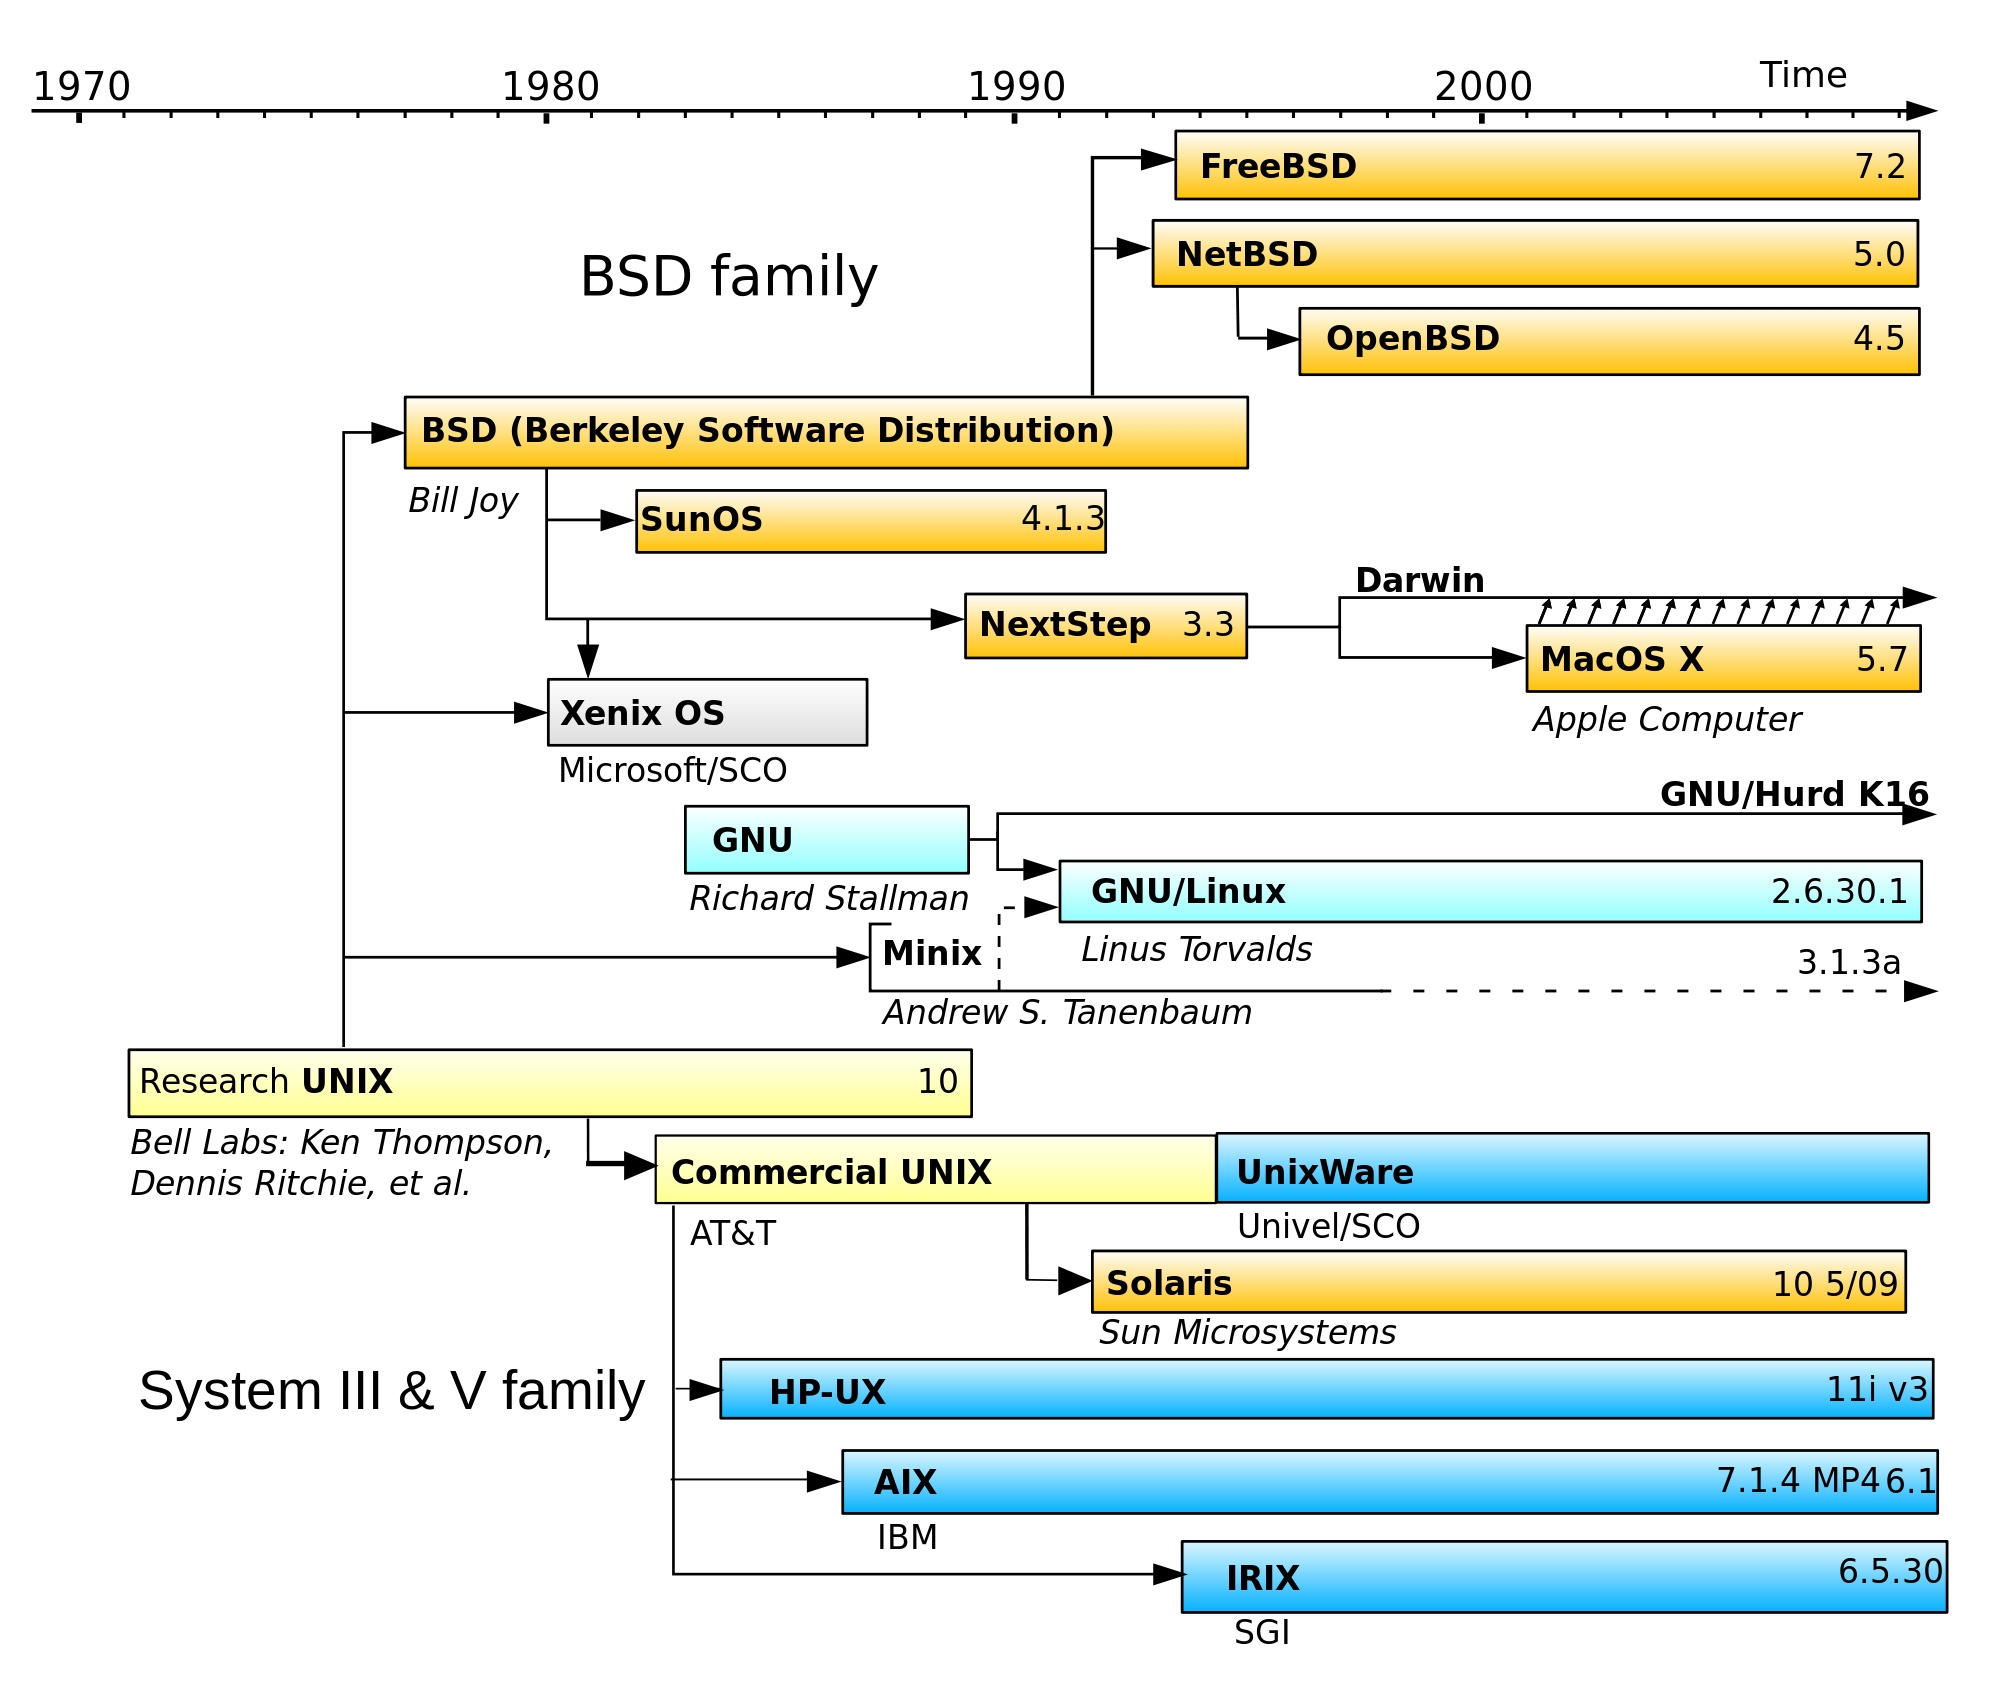
\includegraphics[width=0.8\textwidth]{./Unix_history}
  \end{center}
	}

\begin{frame}
  \frametitle{What is Linux?}
  \begin{itemize}
    \item Linux is an operating system that evolved from a kernel created by Linus Torvalds when he was a student at the University of Helsinki. 
    \item It's meant to be used as an alternative to other operating systems, Windows, Mac OS, MS-DOS, Solaris and others. 
    \item Linux is the most popular OS used in a Supercomputer\let\thefootnote\relax\footnote{\tiny \url{http://www.top500.org/statistics/list/}}
      \begin{center}
  \begin{tikzpicture}
    \node (tbl) {
      \begin{tabularx}{0.42\textwidth}{ccc}
        \arrayrulecolor{black}
        \textcolor{white}{\textbf{OS Family} }& \textcolor{white}{\textbf{Count}} &\textcolor{white}{\textbf {Share \%}}\\
        Linux \rule{0pt}{3.5ex} & 489 & 97.8 \\
        Unix & 9 & 1.8 \\
        Windows & 1 & 0.2 \\
        Mixed & 1 & 0.2 \\
        [1.0ex]
    \end{tabularx}};
    \begin{pgfonlayer}{background}
      %\draw[rounded corners,top color=blue!30!black,bottom color=blue!10!white,
      \draw[rounded corners,top color=lupurple,bottom color=lupurple,
        draw=lubrown!30] ($(tbl.north west)+(0.14,0)$)
      rectangle ($(tbl.north east)-(0.13,0.9)$);
      %\draw[rounded corners,top color=green!5,bottom color=green!5,draw=green!5]
      \draw[rounded corners,top color=lulime,bottom color=lulime,draw=lulime]
      ($(tbl.north east)-(0.13,0.6)$)
      rectangle ($(tbl.south west)+(0.13,0.2)$);
    \end{pgfonlayer}
  \end{tikzpicture}
\end{center}



    \item If you are using a Supercomputer for your research, it will most likely be based on a *nix OS.
  \end{itemize}
\end{frame}

\begin{frame}
  \frametitle{What is Linux?}
  \begin{itemize}
    \item Many software vendors release their own packaged Linux OS (kernel, applications) known as distribution
    \item Linux distribution = Linux kernel + GNU system utilities and libraries + Installation scripts + Management utilities etc.
    \begin{enumerate}
      {%\scriptsize
        \item Debian, Ubuntu, Mint
        \item Red Hat, Fedora, CentOS
        \item Slackware, openSUSE, SLES, SLED
        \item Gentoo
      }
    \end{enumerate}
    \item Application packages on Linux can be installed from source or from customized packages
    \begin{enumerate}
      {%\scriptsize
        \item deb: Debian based distros e.g. Debian, Ubuntu, Mint
        \item rpm: Red Hat based distros, Slackware based distros.
      }
    \end{enumerate}
    \item Linux distributions offer a variety of desktop environment.
    \begin{enumerate}
      {%\scriptsize
        \item K Desktop Environment (KDE)
        \item GNOME 
        \item Xfce
        \item Lightweight X11 Desktop Environment (LXDE)
        \item Cinnamon
        \item MATE
      }
    \end{enumerate}
  \end{itemize}
\end{frame}

\begin{frame}{openSUSE KDE Desktop}
  \begin{center}
    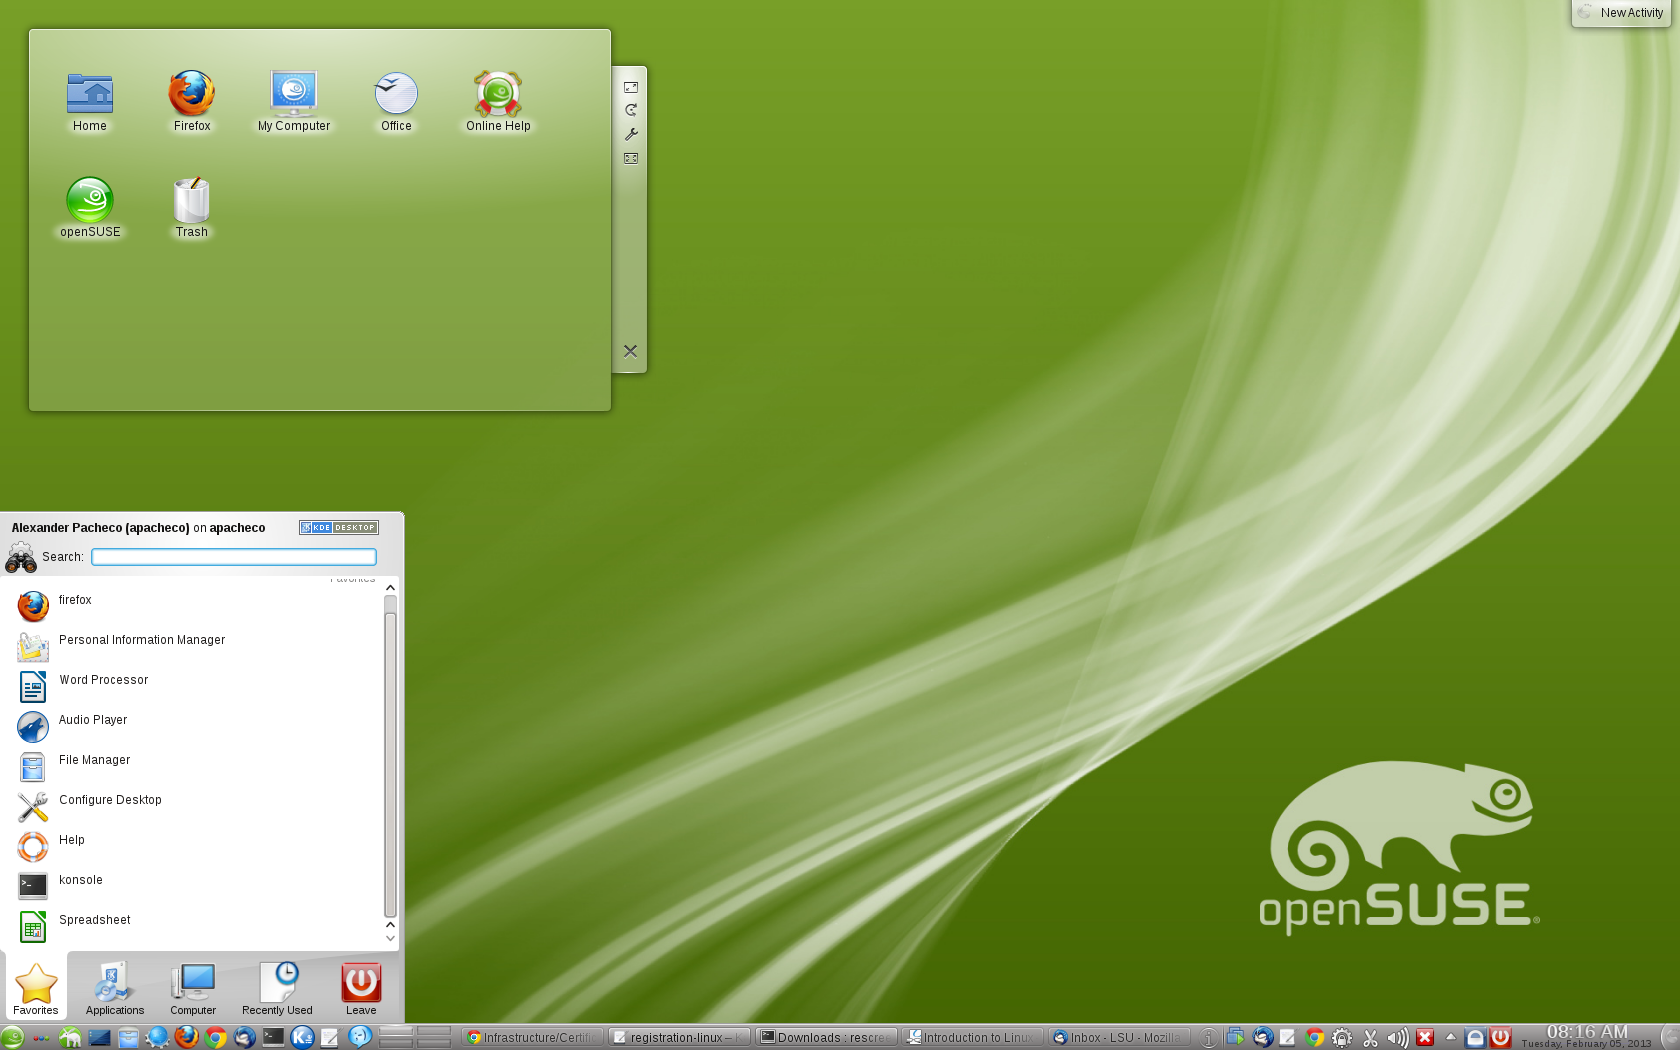
\includegraphics[width=\textwidth]{./opensuse}
  \end{center}
\end{frame}
\begin{frame}{CentOS GNOME Desktop}
  \begin{center}
    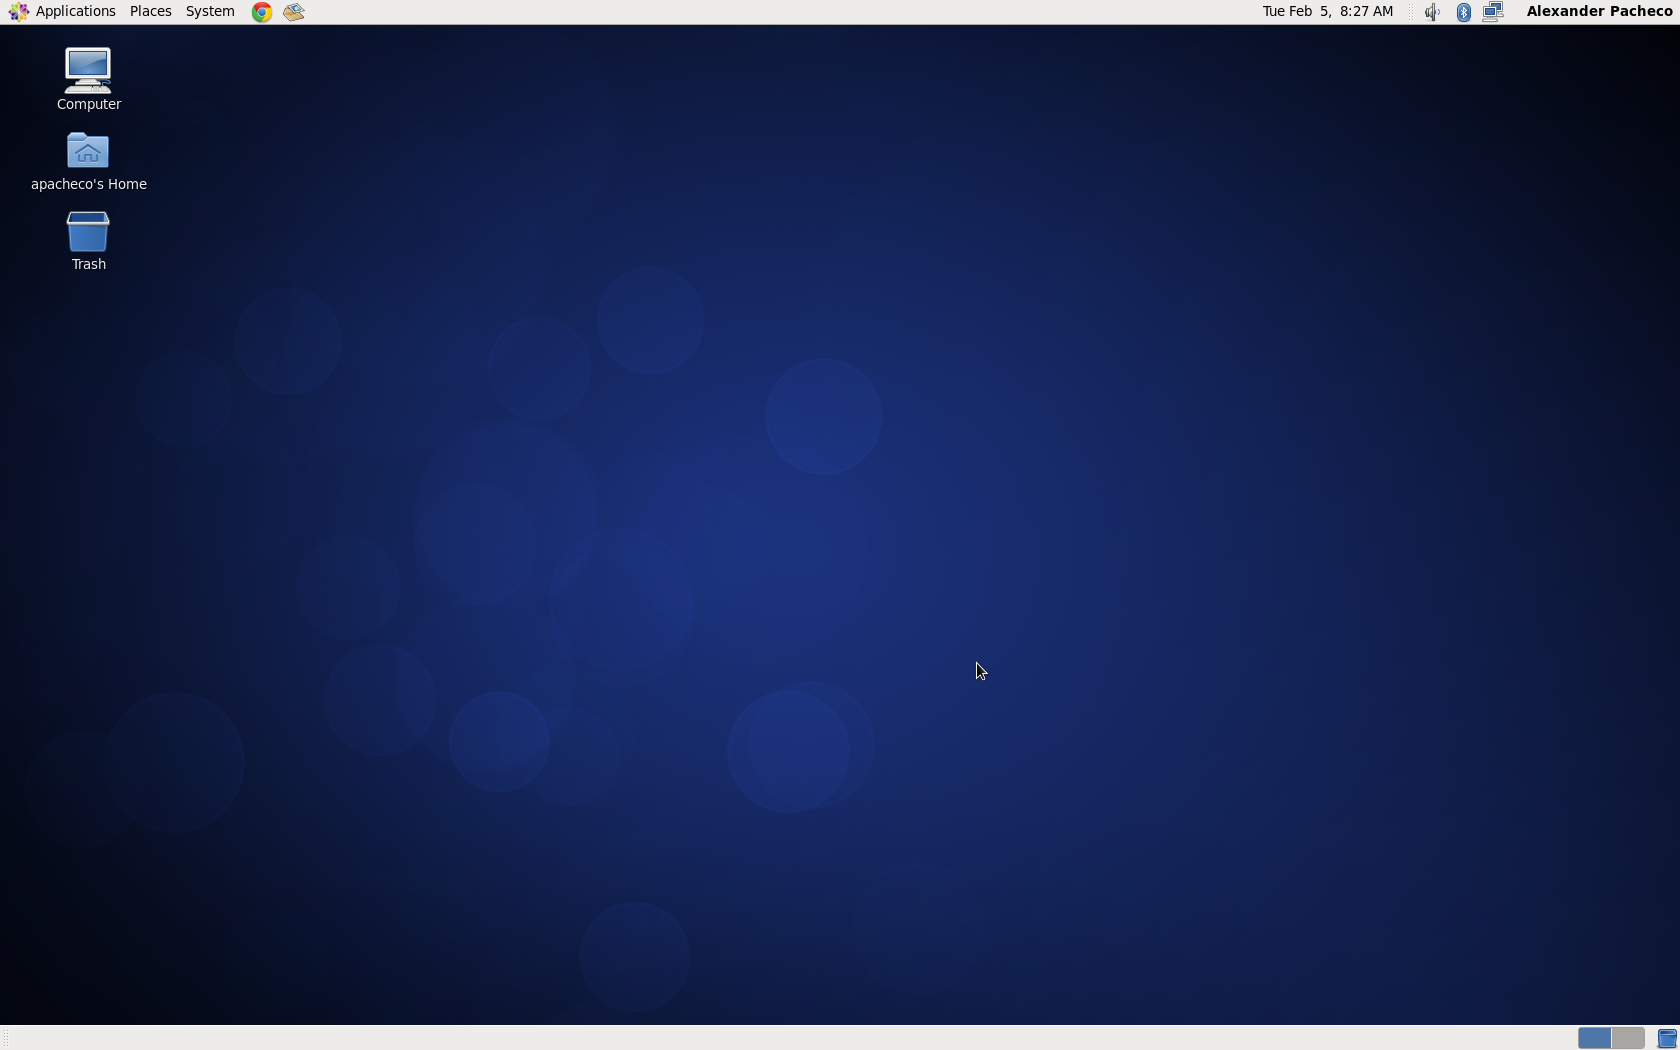
\includegraphics[width=\textwidth]{./CentOS6_3}
  \end{center}
\end{frame}
\begin{frame}{LXDE Desktop}
  \begin{center}
    
\includegraphics[width=0.85\textwidth]{./LXDE_desktop_full}
  \end{center}
\end{frame}
\begin{frame}{Debian MATE Desktop}
  \begin{center}
    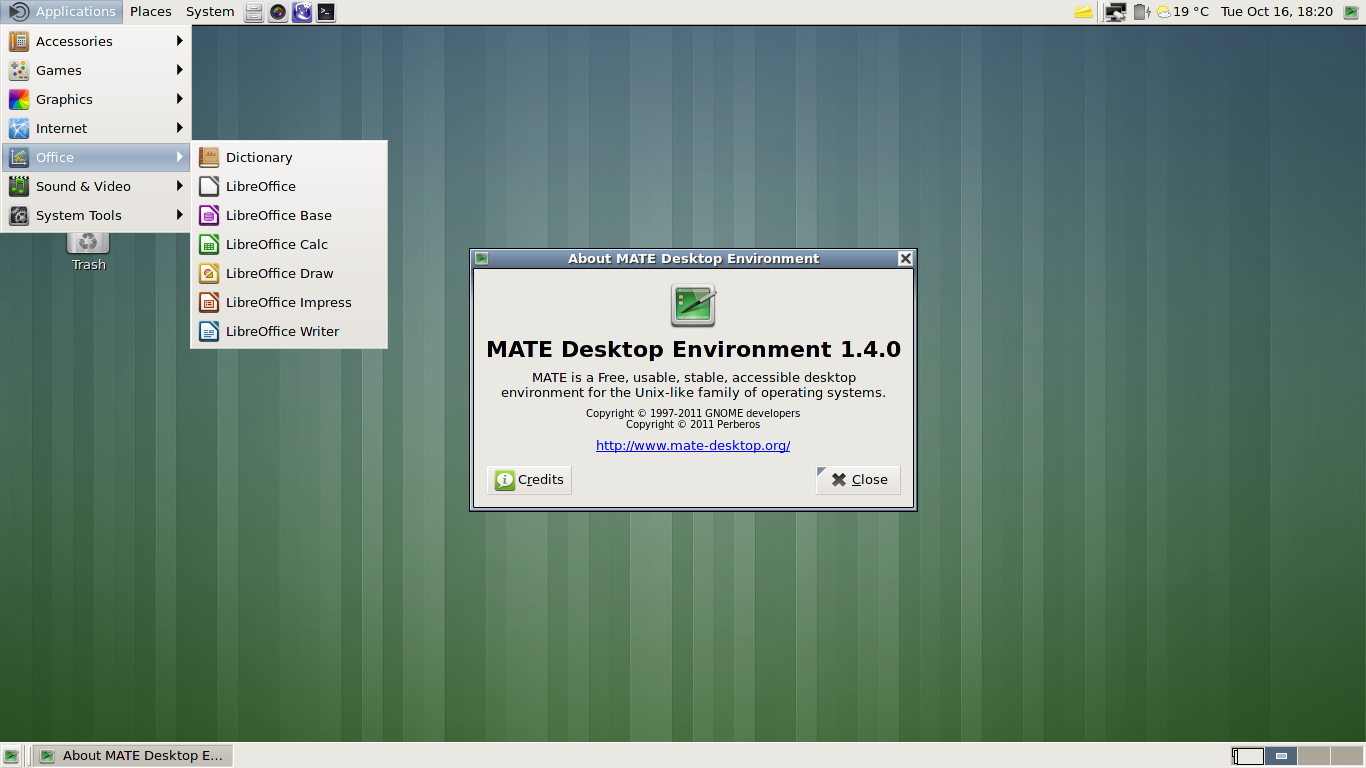
\includegraphics[width=\textwidth]{./Mate_DE_on_Debian}
  \end{center}
\end{frame}
\begin{frame}{Linux Mint Cinnamon Desktop}
  \begin{center}
    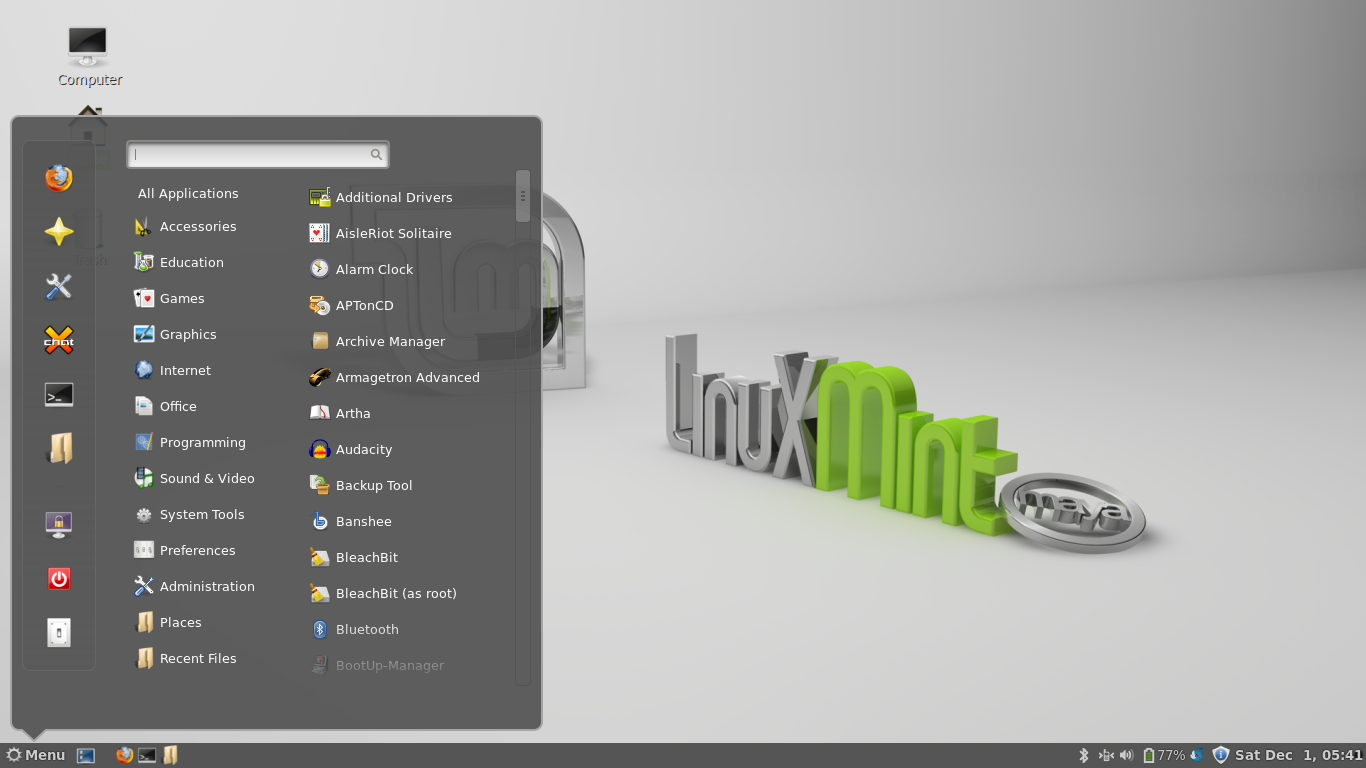
\includegraphics[width=\textwidth]{./Cinnamon_Mint}
  \end{center}
\end{frame}

\begin{frame}
  \frametitle{What is Linux?}
  \begin{itemize}
    \item Linux distributions are tailored to different requirements such as
    \begin{enumerate}
      {%\scriptsize
        \item Server
        \item Desktop
        \item Workstation
        \item Routers
        \item Embedded devices
        \item Mobile devices (Android is a Linux-based OS)
      }
    \end{enumerate}
    \item Almost any software that you use on windows has a roughly equivalent software on Linux, most often multiple equivalent software
    \item[e.g.] Microsoft Office equivalents are OpenOffice.org, LibreOffice, KOffice
    \item For complete list, visit \url{http://wiki.linuxquestions.org/wiki/Linux_software_equivalent_to_Windows_software}
    \item Linux offers you freedom, to choose your desktop environment, software.
  \end{itemize}
\end{frame}

\begin{frame}[fragile]
  \frametitle{Popularity of Linux Distributions}
  \begin{columns}[T]
    \column{0.43\textwidth}
    \begin{itemize}
      \item \href{http://distrowatch.com/}{\color{blue}DistroWatch} provides news, popularity rankings, and other general information about:
      \begin{enumerate}
        {%\scriptsize
          \item various Linux distributions,
          \item free software/open source Unix-like operating systems such as OpenSolaris, MINIX and BSD.
        }
      \end{enumerate}
      \item DistroWatch is NOT an indication of market-share or quality nor is it an indication of how many users but  it is clearly an indication of what users are looking at.
    \end{itemize}
    \column{0.57\textwidth}
    \begin{center}
  {%\scriptsize
    \begin{matrixtable}{1.2cm}{2.4cm}{1.2cm}{0.6cm}{
        \head{Rank} & \head{Distribution} & \head{Hits} & \\
        1 & Mint        & 3105 & \const   \\
        2 & Debian      & 1764 & \up \\
        3 & Ubuntu      & 1603 & \const   \\
        4 & openSUSE    & 1198 & \up   \\
        5 & Fedora      & 1142 & \const   \\
        6 & Mageia      & 1016 & \down   \\
        7 & CentOS      & 970 & \down   \\
        8 & Manjaro     & 943 & \const \\
        9 & LXLE        & 788  & \up   \\
        10& Arch        & 759  & \const   \\
      }
    \end{matrixtable}
  }
\end{center}

  \end{columns}
\end{frame}

\begin{frame}
  \frametitle{Linux Components}
  \begin{columns}[T]
    \column{0.5\textwidth}
    \begin{itemize}
    \item Linux is made up of two (three) parts:
      \begin{enumerate}
      \item Kernel 
      \item Shell 
      \item Applications/Programs 
      \end{enumerate}
    \end{itemize}
    \column{0.5\textwidth}
    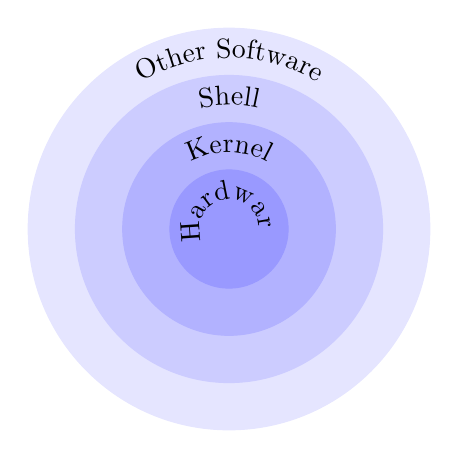
\begin{tikzpicture}[scale=0.75]
      %    \begin{scope}[xshift=6cm]
      \coordinate (O) at (0,0);
      \foreach \k in {1,...,4}\pgfmathparse{10*\k} \draw[fill=blue!\pgfmathresult!white,blue!\pgfmathresult!white] (O) circle (4.2-0.8*\k);
      \foreach \k/\text in {0/{Other Software},1/Shell,2/Kernel,3/Hardware} \draw[decoration={text along path,reverse path,text align={align=center},text={\text}},decorate] (2.9-0.8*\k,0) arc (0:180:2.9-0.8*\k);
      %    \end{scope}
    \end{tikzpicture}
  \end{columns}
\end{frame}
  
\begin{frame}[allowframebreaks]
  \frametitle{Linux Components}
  \begin{columns}[T]
  \column{0.5\textwidth}
  \begin{itemize}
    \item Linux is made up of two (three) parts:
    \begin{enumerate}
      {%\scriptsize
        \item Kernel 
        \item Shell 
        \item Applications/Programs 
        }
    \end{enumerate}
  \end{itemize}
  \column{0.5\textwidth}
  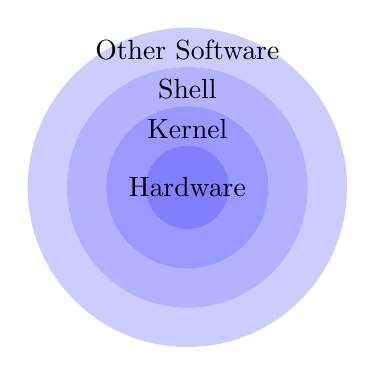
\begin{tikzpicture}
    \draw [fill=blue!20!white, ultra thick, blue!20!white] (3,0) circle (2.0);
    \draw [fill=blue!30!white, ultra thick, blue!30!white] (3,0) circle (1.5);
    \draw [fill=blue!40!white, ultra thick, blue!40!white] (3,0) circle (1.0);
    \draw [fill=blue!50!white, ultra thick, blue!50!white] (3,0) circle (0.5);
    \node at (3,0) {Hardware};
    \node [above] at (3,.5) {Kernel};
    \node [above] at (3,1) {Shell};
    \node [above] at (3,1.5) {Other Software};
  \end{tikzpicture}
  \end{columns}
%  \framebreak
  \begin{block}{What is a kernel}
    \begin{itemize}
      \item The kernel is the main component of most computer operating systems
      \item It is a bridge between applications and the actual data processing done at the hardware level.
      \item The kernel's responsibilities include managing the system's resources (the communication between hardware and software components).
      \item provides the lowest-level abstraction layer for the resources (especially processors and I/O devices) that application software must control to perform its function.
      \item It typically makes these facilities available to application processes through inter-process communication mechanisms and system calls.
    \end{itemize}
  \end{block}
  \begin{exampleblock}{What is a SHELL}
    \begin{itemize}
      \item The command line interface is the primary interface to Linux/Unix operating systems.
      \item Shells are how command-line interfaces are implemented in Linux/Unix.
      \item Each shell has varying capabilities and features and the user should choose the shell that best suits their needs.
      \item The shell is simply an application running on top of the kernel and provides a powerful interface to the system.
    \end{itemize}
  \end{exampleblock}
\end{frame}

\begin{frame}
  \frametitle{Types of Shell}
    \begin{itemize}
      \item[\texttt{sh}]: Bourne Shell
      \begin{enumerate}
        {%\scriptsize
          \item[$\vardiamond$] Developed by Stephen Bourne at AT\&T Bell Labs
        }
      \end{enumerate}
      \item[\texttt{csh}]: C Shell
      \begin{enumerate}
        {%\scriptsize
          \item[$\vardiamond$] Developed by Bill Joy at University of California, Berkeley
        }
      \end{enumerate}
      \item[\texttt{ksh}]: Korn Shell
      \begin{enumerate}
        {%\scriptsize
          \item[$\vardiamond$] Developed by David Korn at AT\&T Bell Labs
          \item[$\vardiamond$] backward-compatible with the Bourne shell and includes many features of the C shell
        }
      \end{enumerate}
      \item[\texttt{bash}]: Bourne Again Shell
      \begin{enumerate}
        {%\scriptsize
          \item[$\vardiamond$] Developed by Brian Fox for the GNU Project as a free software replacement for the Bourne shell (sh).
          \item[$\vardiamond$] Default Shell on Linux and Mac OSX
          \item[$\vardiamond$] The name is also descriptive of what it did, bashing together the features of sh, csh and ksh
        }
      \end{enumerate}
      \item[\texttt{tcsh}]: TENEX C Shell
      \begin{enumerate}
        {%\scriptsize
          \item[$\vardiamond$] Developed by Ken Greer at Carnegie Mellon University 
          \item[$\vardiamond$] It is essentially the C shell with programmable command line completion, command-line editing, and a few other features.
        }
      \end{enumerate}
    \end{itemize}
\end{frame}

\begin{frame}
  \frametitle{Shell Comparison}
  \begin{columns}
    \column{0.65\textwidth}
    \begin{center}
      \begin{tikzpicture}
        \node (tbl) {
          \begin{tabularx}{\textwidth}{cccccc}
            \arrayrulecolor{black}
            \textcolor{white}{\textbf{Software} }& \textcolor{white}{\textbf{sh}} &\textcolor{white}{\textbf {csh}} & \textcolor{white}{\textbf{ksh}} & \textcolor{white}{\textbf{bash}} & \textcolor{white}{\textbf{tcsh}} \\
            Programming Language\rule{0pt}{3.5ex} & \cmark & \cmark & \cmark & \cmark & \cmark \\
            Shell Variables & \cmark & \cmark & \cmark & \cmark & \cmark \\
            Command alias & \xmark & \cmark & \cmark & \cmark & \cmark \\
            Command history & \xmark & \cmark & \cmark & \cmark & \cmark \\
            Filename completion & \xmark & \smark & \smark & \cmark & \cmark \\
            Command line editing & \xmark & \xmark & \smark & \cmark & \cmark \\
            Job control & \xmark & \cmark & \cmark & \cmark & \cmark \\
            [1.0ex]
        \end{tabularx}};
        \begin{pgfonlayer}{background}
          %\draw[rounded corners,top color=blue!30!black,bottom color=blue!10!white,
          \draw[rounded corners,top color=lupurple,bottom color=lupurple,
            draw=lubrown!30] ($(tbl.north west)+(0.14,0)$)
          rectangle ($(tbl.north east)-(0.13,0.9)$);
          %\draw[rounded corners,top color=black,bottom color=lubrown!20,
          %   middle color=lubrown!20,draw=lubrown!20] ($(tbl.south west)
          %   +(0.12,0.5)$) rectangle ($(tbl.south east)-(0.12,0)$);
          %\draw[rounded corners,top color=green!5,bottom color=green!5,draw=green!5]
          \draw[rounded corners,top color=lulime,bottom color=lulime,draw=lulime]
          ($(tbl.north east)-(0.13,0.6)$)
          rectangle ($(tbl.south west)+(0.13,0.2)$);
        \end{pgfonlayer}
      \end{tikzpicture}
      \begin{itemize}
        \item[\cmark]: Yes
        \item[\xmark]: No
        \item[\smark]: Yes, not set by default
        \item[] {\fontsize{6}{7}\selectfont\url{http://www.cis.rit.edu/class/simg211/unixintro/Shell.html}}
      \end{itemize}
    \end{center}
  \end{columns}
\end{frame}

\begin{frame}
  \frametitle{\small Start Up Scripts}
  \begin{itemize}
    \item When you login to a *NIX computer, shell scripts are automatically loaded depending on your default \textbf{\color{lubrown}shell}
    \item \textbf{\color{lubrown}sh,ksh}
    \begin{enumerate}
        \item \texttt{\color{blue}/etc/profile}
        \item \texttt{\color{blue}\$HOME/.profile}
    \end{enumerate}
    \item \textbf{\color{lubrown}bash}
    \begin{enumerate}
        \item \texttt{\color{blue}/etc/profile}, login terminal only
        \item \texttt{\color{blue}/etc/bashrc} or \texttt{\color{blue}/etc/bash/bashrc}
        \item \texttt{\color{blue}\$HOME/.bash\_profile}, login terminal only
        \item \texttt{\color{blue}\$HOME/.bashrc}
    \end{enumerate}
    \item \textbf{\color{lubrown}csh,tcsh}
    \begin{enumerate}
        \item \texttt{\color{blue}/etc/csh.cshrc}
        \item \texttt{\color{blue}\$HOME/.tcshrc}
        \item \texttt{\color{blue}\$HOME/.cshrc} if .tcshrc is not present
    \end{enumerate}
    \item The \texttt{\color{blue}.bashrc, .tcshrc, .cshrc, .bash\_profile} are script files where users can define their own aliases, environment variables, modify paths etc.
    %\item e.g. the \textbf{\color{lubrown}alias} command covered earlier can be put in one of these script files depending on your \textbf{\color{lubrown}shell}
  \end{itemize}
\end{frame}

\begin{frame}[fragile, allowframebreaks]
  \frametitle{\small Examples}
  \begin{lstlisting}[language=bash,basicstyle=\tiny\ttfamily]
# .bashrc

# Source global definitions
if [ -f /etc/bashrc ]; then
        . /etc/bashrc
fi

# User specific aliases and functions
alias c="clear"
alias rm="/bin/rm -i"
alias psu="ps -u apacheco"
alias em="emacs -nw"
alias ll="ls -lF"
alias la="ls -al"
export PATH=/home/apacheco/bin:${PATH}
export g09root=/home/apacheco/Software/Gaussian09
export GAUSS_SCRDIR=/home/apacheco/Software/scratch
source $g09root/g09/bsd/g09.profile

export TEXINPUTS=.:/usr/share/texmf//:/home/apacheco/LaTeX//:${TEXINPUTS}
export BIBINPUTS=.:/home/apacheco/TeX//:${BIBINPUTS}
  \end{lstlisting}

  \begin{lstlisting}[language=csh,basicstyle=\tiny\ttfamily]
# .tcshrc

# User specific aliases and functions
alias c clear
alias rm "/bin/rm -i"
alias psu "ps -u apacheco"
alias em "emacs -nw"
alias ll "ls -lF"
alias la "ls -al"
setenv PATH "/home/apacheco/bin:${PATH}"
setenv g09root "/home/apacheco/Software/Gaussian09"
setenv GAUSS_SCRDIR "/home/apacheco/Software/scratch"
source $g09root/g09/bsd/g09.login

setenv TEXINPUTS ".:/usr/share/texmf//:/home/apacheco/LaTeX//:${TEXINPUTS}"
setenv BIBINPUTS ".:/home/apacheco/TeX//:${BIBINPUTS}"
  \end{lstlisting}
\end{frame}

\begin{frame}
  \frametitle{Files and Processes}
  \begin{itemize}
    \item Everything in Linux/UNIX is either a file or a process
    \item A File is a collection of data, created by users using text editors, running compilers, etc.
    \item Examples of Files:
    \begin{enumerate}
      {%\scriptsize
        \item document such as collection of ascii text as in report, essay, etc. 
        \item program written in some high level programming language
        \item instructions comprehensible to machine but not a casual user such as executable, binary file
        \item directory containing information about its contents such as subdirectories or other files
      }
    \end{enumerate}
    \item A process is an executing program identified by a unique process identifier or PID.
  \end{itemize}
\end{frame}

%% Tikz File System Heirarchy
 \tikzset{
    invisible/.style={opacity=0},
    visible on/.style={alt={#1{}{invisible}}},
    alt/.code args={<#1>#2#3}{%
      \alt<#1>{\pgfkeysalso{#2}}{\pgfkeysalso{#3}} % \pgfkeysalso doesn't change the path
    },
  }

\begin{frame}{File System Hierarchy}
\tikzset{every node/.append style={scale=0.4}}

\begin{tikzpicture}[scale=0.4]
  \path[mindmap,concept color=lubrown,text=lucream,
  level 1 concept/.append style={every child/.style={concept color=luorange,text=black},sibling angle=-15},
  level 2 concept/.append style={every child/.style={concept color=luorange2,text=black}, sibling angle=-40},
  level 3 concept/.append style={every child/.style={concept color=lulime,text=black}}]
    node[concept] {root directory (/)}
    [clockwise from=180]
    child[style={concept}, level distance=8.5cm, visible on=<2->] { node[concept] {bin}}
    child[concept, visible on=<3->] { node[concept] {boot}}
    child[style={concept}, level distance=8.5cm, visible on=<4->] { node[concept] {dev}}
    child[concept, visible on=<5->] { node[concept] {etc}}
    child[style={concept}, level distance=8.5cm, visible on=<6->] { node[concept] {home}
		[counterclockwise from=-90]
      	child { node[concept] {alp514} 
        	[clockwise from=0]
            child { node[concept] {.bashrc}}
            child { node[concept] {bin}}
            child { node[concept] {Documents}}
            child { node[concept] {packages}}
            child { node[concept] {$\cdots$}}
        }
      	child[visible on=<16->] { node[concept] {sma310} }
      	child[visible on=<16->] { node[concept] {$\cdots$} }
	}
    child[concept, visible on=<7->] { node[concept] {lib64 \& lib}}
    child[style={concept}, level distance=8.5cm, visible on=<8->] { node[concept] {mnt}}
    child[concept, visible on=<9->] { node[concept] {proc}}
    child[style={concept}, level distance=8.5cm, visible on=<10->] { node[concept] {sbin}}
    child[concept, visible on=<11->] { node[concept] {tmp}}
    child[style={concept}, level distance=11.5cm, visible on=<12->] { node[concept] {usr}
		[counterclockwise from=15]
      	child { node[concept] {bin} }
      	child { node[concept] {lib64 \& lib} }
      	child { node[concept] {local} }
      	child { node[concept] {include} }
      	child { node[concept] {sbin} }
      	child { node[concept] {share} }
        }
    child[concept, visible on=<13->] { node[concept] {var}}
    child[style={concept}, level distance=8.5cm, visible on=<14->] { node[concept] {zhome}
		[counterclockwise from=0]
      	child { node[concept] {Apps} 
        	[clockwise from=50]
            child { node[concept] {matlab}}
            child { node[concept] {gcc}}
            child { node[concept] {intel}}
            child { node[concept] {pgi}}
        }
      	child { node[concept] {alp514} }
      	child { node[concept] {sma310} }
      	child { node[concept] {$\cdots$} }
	}
;
\end{tikzpicture}

\begin{itemize}
\only<1>{\item All files are arranged in a hierarchial structure, like an inverted tree.}
\only<1>{\item The top of the hierarchy is traditionally called \textbf{root} (written as a slash / )}
\only<2>{\item contains files that are essential for system operation, available for use by all users.}
\only<3>{\item contains bootable kernel and bootloader}
\only<4>{\item contains various devices such as hard disk, CD-ROM drive etc}
\only<5>{\item contains various system configurations}
\only<6>{\item contains home directories of all users. This is the directory where you are at when you login to a Linux/UNIX system.}
\only<7>{\item contains libraries that are essential for system operation, available for use by all users.}
\only<8>{\item directories where disk drives are mounted}
\only<9>{\item process information pseudo-file system containing runtime system information (e.g. system memory, devices mounted, hardware configuration, etc).}
\only<9>{\item can be regarded as a control and information centre for the kernel.}
\only<10>{\item same as bin but only accessible by \textbf{root}}
\only<11>{\item temporary file storage}
\only<12>{\item contains user documentations, binaries, libraries etc}
\only<13>{\item used to store files which change frequently (system level not user level)}
\only<14>{\item where we install applications common to all HPC systems}
\only<15>{\item Installing your own OS: /bin,/lib\{64\},/etc,/dev and /sbin must be on the same partition.}
\only<16>{\item UNIX like OS's are designed for multi user environments i.e. multiple users can exist on the system.}
\only<16>{\item Special user called \textbf{root} is the administrator and has access to all files in the system.}
\end{itemize}
\end{frame}



\begin{frame}
\tikzset{every node/.append style={scale=0.25}}
\begin{tikzpicture}[scale=0.25]
  \path[mindmap,concept color=lubrown,text=white,
  level 1 concept/.append style={every child/.style={concept color=lubrown},sibling angle=-30},
  level 2 concept/.append style={every child/.style={concept color=lubrown},sibling angle=-40}]
    node[concept] {root directory (/)}
    [counterclockwise from=90]
    child[concept color=lubrown] { node[concept] {bin}}
    child[concept color=lubrown] { node[concept] {boot}}
    child[concept color=lubrown] { node[concept] {dev}}
    child[concept color=lubrown] { node[concept] {etc}}
    child[style={concept}, level distance=6.5cm] { node[concept] {home}
		[counterclockwise from=-20]
      	child { node[concept] {alp514} 
        	[clockwise from=90]
            child { node[concept] {.bashrc}}
            child { node[concept] {bin}}
            child { node[concept] {Documents}}
            child { node[concept] {packages}}
            child { node[concept] {$\cdots$}}
        }
      	child { node[concept] {sma310} }
      	child { node[concept] {$\cdots$} }
	}
    child[concept color=lubrown] { node[concept] {lib64 \& lib}}
    child[concept color=lubrown] { node[concept] {mnt}}
    child[concept color=lubrown] { node[concept] {sbin}}
    child[concept color=lubrown] { node[concept] {tmp}}
    child[style={concept}, level distance=6.5cm] { node[concept] {usr}
		[clockwise from=90]
      	child { node[concept] {bin} }
      	child { node[concept] {lib64 \& lib} }
      	child { node[concept] {local} }
      	child { node[concept] {include} }
      	child { node[concept] {sbin} }
        }
    child[concept color=lubrown] { node[concept] {var}}
    child[style={concept}, level distance=6.5cm] { node[concept] {zhome}
		[clockwise from=40]
      	child { node[concept] {Apps} }
      	child { node[concept] {alp514} }
      	child { node[concept] {sma310} }
      	child { node[concept] {$\cdots$} }
	}
;
\end{tikzpicture}
\end{frame}

\begin{frame}
  \frametitle{Directory Structure}
%    \vspace{-0.5cm}
  \begin{itemize}
    \item All files are arranged in a hierarchial structure, like an inverted tree.
    \item The top of the hierarchy is traditionally called \textbf{root} (written as a slash / )
  \end{itemize}
\tikzstyle{every node}=[draw=black,thick,anchor=west]
\tikzstyle{selected}=[draw=red,fill=red!30]
\tikzstyle{optional}=[dashed,fill=gray!50]
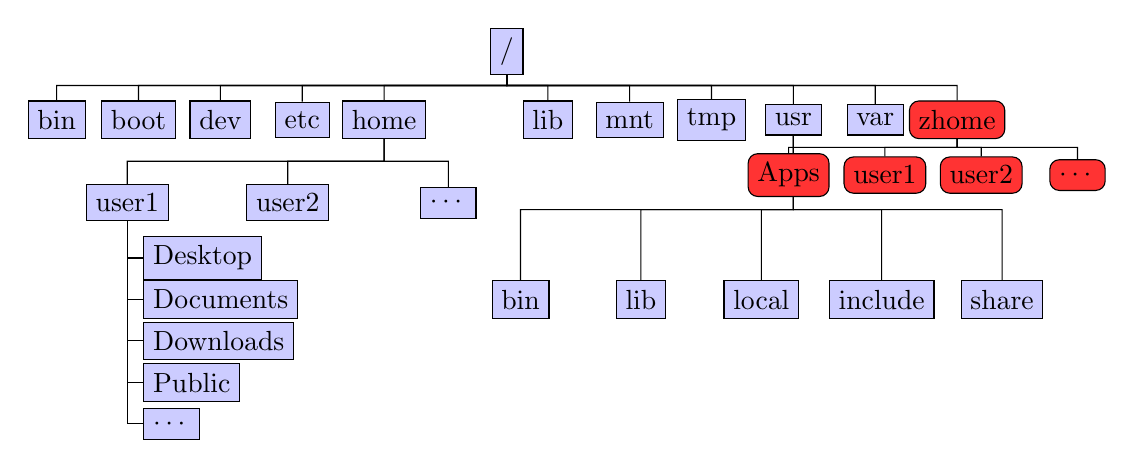
\begin{tikzpicture}[%
  linux/.style={rectangle,draw,fill=blue!20},
  hpc/.style={rectangle,draw,fill=red!80,rounded corners=.8ex},
  grandchild/.style={grow=down,xshift=1em,anchor=west,
    edge from parent path={(\tikzparentnode.south) |- (\tikzchildnode.west)}},
  first/.style={level distance=12ex,sibling distance=10em,xshift=-6em},
  second/.style={level distance=8ex,sibling distance=6em,xshift=-1.5em},
  third/.style={level distance=26ex,sibling distance=7.5em,xshift=-2em},
  fourth/.style={level distance=8ex},
  fifth/.style={level distance=14ex},
  sixth/.style={level distance=20ex},
  seventh/.style={level distance=26ex},
  eighth/.style={level distance=32ex},
  level 1/.style={sibling distance=5.1em},
  scale=0.58]
    % Parents
    \coordinate
    child[grow=down,level distance=0ex]{node[linux]{ / }}
    [edge from parent fork down]
    % Children and grandchildren
    child {node[linux] {bin}}
    child {node[linux] {boot}}
    child {node[linux] {dev}}
    child {node[linux] {etc}}
    child {node[linux] {home}
      child [first] {node[linux] {user1}
          child[grandchild,fourth] {node[linux] {Desktop}}
          child[grandchild,fifth] {node[linux] {Documents}}
          child[grandchild,sixth] {node[linux] {Downloads}}
          child[grandchild,seventh] {node[linux] {Public}}
          child[grandchild,eighth] {node[linux] {$\cdots$}}
       }
      child [first] {node[linux] {user2}
       }
      child [first] {node[linux] {$\cdots$}}
    }
    child [missing] {}
    child {node[linux] {lib}}
    child {node[linux] {mnt}}
    child {node[linux] {tmp}}
    child {node[linux] {usr}
      child [third] {node[linux] {bin}}
      child [third] {node[linux] {lib}}
      child [third] {node[linux] {local}}
      child [third] {node[linux] {include}}
      child [third] {node[linux] {share}}
    }
    child {node[linux] {var}}
    child {node[hpc] {zhome}
      child [second] {node[hpc] {Apps}}
      child [second] {node[hpc] {user1}}
      child [second] {node[hpc] {user2}}
      child [second] {node[hpc] {$\cdots$}}
    };
\end{tikzpicture}
\end{frame}

\begin{frame}
  \frametitle{Important Directories}
  \begin{description}
    \item[/bin:] contains files that are essential for system operation, available for use by all users.
    \item[/lib,/lib64:] contains libraries that are essential for system operation, available for use by all users.
    \item[/var:] used to store files which change frequently (system level not user level)
    \item[/etc:] contains various system configurations
    \item[/dev:] contains various devices such as hard disk, CD-ROM drive etc
    \item[/sbin:] same as bin but only accessible by \textbf{root}
    \item[/tmp:] temporary file storage
    \item[/boot:] contains bootable kernel and bootloader
    \item[/usr:] contains user documentations, binaries, libraries etc
    \item[/home:] contains home directories of all users. This is the directory where you are at when you login to a Linux/UNIX system.
  \end{description}
  \begin{itemize}
    \item Installing your own OS: /bin,/lib\{64\},/etc,/dev and /sbin must be on the same partition.
  \end{itemize}
\end{frame}

\begin{frame}[fragile]
  \frametitle{\small }
  \begin{itemize}
    \item UNIX like OS's are designed for multi user environments i.e. multiple users can exist on the system.
    \item Special user called \textbf{root} is the administrator and has access to all files in the system.
    \item In *nix, users are organized into groups.
    \item Each user is in alteast one group.
    \item Group membership makes it easier to share files with members of your group.
    \item[]Type \Verblubrown{groups{\Enter}} to find your group membership.
    \item All files are \textit{case sensitive},
    \item[$\vardiamond$] myfile.txt, Myfile.txt and myfile.TXT are three different files and can exist in the same directory simultaneously.
  \end{itemize}
\end{frame}

\begin{frame}
  \frametitle{Relative \& Absolute Path}
  \begin{itemize}
    \item \textit{Path} means a position in the directory tree.
    \item You can use either the \textit{relative path} or \textit{absolute path}
    \item In \textit{relative path} expression
    \begin{itemize}
      {%\scriptsize
        \item . (one dot or period) is the current working directory
        \item .. (two dots or periods) is one directory up
        \item You can combine . and .. to navigate the file system hierarchy.
        \item the path is not defined uniquely and does depend on the current path.
        \item \texttt{../../tmp} is unique only if your current working directory is your home directory.
      }
    \end{itemize}
    \item In \textit{absolute path} expression 
    \begin{itemize}
      {%\scriptsize
        \item the path is defined uniquely and does not depend on the current path
        \item \texttt{/tmp} is unique since /tmp is the \textit{abolute path}
      }
    \end{itemize}
  \end{itemize}
\end{frame}


\section{Variables}
\begin{frame}[fragile,allowframebreaks]
  \frametitle{Variables}
  \begin{itemize}
    \item *nix also permits the use of variables, similar to any programming language such as C, C++, Fortran etc
    \item A variable is a named object that contains data used by one or more applications. 
    \item There are two types of variables, Environment and User Defined and can contain  a number, character or a string of characters.
    \item Environment Variables provides a simple way to share configuration settings between multiple applications and processes in Linux.
    \item By Convention, enviromental variables are often named using all uppercase letters
    \item[e.g.] \Verblubrown{PATH, LD\_LIBRARY\_PATH, LD\_INCLUDE\_PATH, TEXINPUTS,} etc
    \item To reference a variable (environment or user defined) prepend \$ to the name of the variable
    \item[e.g.] \Verblubrown{\$PATH, \$LD\_LIBRARY\_PATH}
    \framebreak
  \end{itemize}
%\end{frame}
%
%\begin{frame}[allowframebreaks]
%  \frametitle{\small Environment Variable}
  \begin{itemize}
    \item The command \Verblubrown{printenv} list the current environmental variables.
    \item[$\mybigstar$] {Type \Verblubrown{printenv} on your command prompt to list all environment variables in your current session.}
    \item The command \Verblubrown{env} is used to either print a list of environment variables or run another utility in an altered environment without having to modify the currently existing environment.
    \item[$\mybigstar$] {Type \Verblubrown{env SHELL=/bin/tcsh xterm} to start an xterm session in tcsh}
    \item[$\vardiamond$] {To execute the above command successfully, you need to be in GUI mode on the virtual OS or logged into a remote systems with X-Forwarding enabled.}
  \end{itemize}
  \framebreak
  \begin{description}
    \item[PATH:] A list of directory paths.
    \item[HOME:] indicate where a user's home directory is located in the file system.
    \item[PWD:] contains path to current working directory.
    \item[OLDPWD:] contains path to previous working directory.
    \item[TERM:] specifies the type of computer terminal or terminal emulator being used
    \item[SHELL:] contains name of the running, interactive shell.
    \item[PS1:] default command prompt
    \item[PS2:] secondary command prompt
    \item[LD\_LIBRARY\_PATH:] colon-separated set of directories where libraries should be searched for first
    \item[HOSTNAME:] The systems host name
    \item[USER:] Current logged in user's name
    \item[DISPLAY:] Network name of the X11 display to connect to, if available.
%    \item[LD\_INCLUDE\_PATH:] 
  \end{description}
  \framebreak
  \begin{itemize}
    \item You can edit the environment variables.
    \item Command to do this depends on the shell
    \item[$\mybigstar$] To add your bin directory to the \Verblubrown{PATH} variable
    \item[] \Verblubrown{sh/ksh/bash}: \Verblubrown{export PATH=\$\{HOME\}/bin:\$\{PATH\}}
    \item[] \Verblubrown{csh/tcsh}: \Verblubrown{setenv PATH \$\{HOME\}/bin:\$\{PATH\}}
    \item[$\mybigstar$] Note the syntax for the above commands
    \item[$\mybigstar$] \Verblubrown{sh/ksh/bash:} {no spaces except between \Verblubrown{export} and \Verblubrown{PATH}}
    \item[$\mybigstar$] \Verblubrown{csh,tcsh:} {no = sign, just a space between \Verblubrown{PATH} and the absolute path}
    \item[$\mybigstar$] \Verblubrown{all shells:} {colon(:) to separate different paths and the variable that is appended to}
    \item \textbf{Yes, the order matters.} If you have a customized version of a software say perl in your home directory, if you append the perl path to \Verblubrown{PATH} at the end, your program will use the system wide perl not your locally installed version.
      \framebreak
    \item Rules for Variable Names
    \begin{enumerate}
      {%\scriptsize
        \item Variable names must start with a letter or underscore
        \item Number can be used anywhere else
        \item DO NOT USE special characters such as \texttt{@, \#, \%, \$}
        \item Case sensitive
        \item Examples
        \begin{itemize}
          {%\scriptsize
          \item Allowed: VARIABLE, VAR1234able, var\_name, \_VAR
          \item Not Allowed: 1VARIABLE, \%NAME, \$myvar, VAR@NAME 
          }
        \end{itemize}
      }
    \end{enumerate}
    \item Assigning value to a variable
    \begin{center}
      \begin{tikzpicture}
        \node (tbl) {
          \begin{tabularx}{0.65\textwidth}{ccc}
            \arrayrulecolor{black}
            \textcolor{white}{\textbf{Type} }& \textcolor{white}{\textbf{sh,ksh,bash}} &\textcolor{white}{\textbf {csh,tcsh}}\\
            Shell \rule{0pt}{3.5ex} & name=value & set name = value \\
            Environment & export name=value & setenv name value \\
            [1.0ex]
        \end{tabularx}};
        \begin{pgfonlayer}{background}
          \draw[rounded corners,top color=lupurple,bottom color=lupurple,
            draw=lubrown!30] ($(tbl.north west)+(0.14,0)$)
          rectangle ($(tbl.north east)-(0.13,0.9)$);
          \draw[rounded corners,top color=lulime,bottom color=lulime,draw=lulime]
          ($(tbl.north east)-(0.13,0.6)$)
          rectangle ($(tbl.south west)+(0.13,0.2)$);
        \end{pgfonlayer}
      \end{tikzpicture}
    \end{center}
    \item \Verblubrown{sh,ksh,bash} THERE IS NO SPACE ON EITHER SIDE OF =
    \item \Verblubrown{csh,tcsh} space on either side of = is allowed for the \Verblubrown{set} command
    \item \Verblubrown{csh,tcsh} There is no = in the \Verblubrown{setenv} command
  \end{itemize}
  \framebreak
  \begin{exampleblock}{Exercise}
    \begin{itemize}
      \item Create two shell variables containing
      \begin{enumerate}
        {%\footnotesize
          \item your name
          \item[e.g.] MYNAME=Alex
          \item a standard greeting
          \item[e.g.] Greet=Hello
        }
      \end{enumerate}
      \item We'll make use of this variables in a few slides when we learn some basic commands.
    \end{itemize}
  \end{exampleblock}
\end{frame}


\section{Basic Commands}
\begin{frame}[fragile]
  \frametitle{Basic Commands}
  \begin{exampleblock}{What is a command and how do you use it?}
    \begin{itemize}
      \item \textbf{command} is a directive to a computer program acting as an interpreter of some kind, in order to perform a specific task.
      \item \textbf{command prompt} (or just \textbf{prompt}) is a sequence of (one or more) characters used in a command-line interface to indicate readiness to accept commands.
      \item Its intent is to literally prompt the user to take action. 
      \item A prompt usually ends with one of the characters \$, \%, \#, :, $>$ and often includes other information, such as the path of the current working directory.
      \item[$\mybigstar$] Virtual Image: \Verb[formatcom=\color{lubrown},fontseries=b,commandchars=\\\{\}]|[user@localhost ~]\$|
%      \item[$\mybigstar$] QueenBee: \texttt{[apacheco@qb4 $\sim$]\$}
      \item[$\mybigstar$] Mac OSX in \Verblubrown{tcsh}: \Verb[formatcom=\color{lubrown},fontseries=b,commandchars=\\\{\}]|[c8-bc-c8-ee-b8-9e:~] apacheco\%|
      \item Each \textbf{command} consists of three parts: name, options, arguments
      \item[] \Verb[formatcom=\color{lubrown},fontseries=b,commandchars=\\\{\}]|[user@localhost ~]\$ command options arguments|
    \end{itemize}
  \end{exampleblock}
\end{frame}

\begin{frame}[fragile]{How to get more information with Linux}
  \begin{itemize}
    \item \Verblubrown{man} shows the manual for a command or program.
    \item The manual is a file that shows you how to use the command and list the different options for the command in question.
    \item Usage: \Verblubrown{man [command]}
    \item Example: \Verblubrown{man ls{\Enter}}
    \item \Verblubrown{apropos} shows you all of the man pages that may shed some light on a certain command.
    \item Usage: \Verblubrown{appropos [keyword]}
    \item Example: \Verblubrown{appropos editor{\Enter}}
  \end{itemize}
% leave space for info command
\end{frame}



\begin{frame}[fragile,allowframebreaks]
  \frametitle{Input \& Output Commands}
  \begin{itemize}
    \item The basis I/O statements are \Verblubrown{echo} for displaying output to screen and \Verblubrown{read} for reading input from screen/keyboard/prompt
    \item The \Verblubrown{read} statement takes all characters typed until the \Verblubrown{{\Enter}} key is pressed and stores them into a variable.
    \item Usage: \Verblubrown{read <variable name>}
    \item Example: \Verblubrown{read name{\Enter}}
    \item[] \Verbblue[it]{Alex Pacheco{\Enter}}
    \item In the above example, the name that you enter in stored in the variable \Verblubrown{name}.
    \item[]
    \item The \Verblubrown{echo arguments} command will print \Verblubrown{arguments} to screen or standard output. 
    \item \Verblubrown{arguments} can be a (single or multiple) variable, string of characters or numbers.
      \framebreak
    \item Examples:
      \begin{enumerate}
        {%\footnotesize
          \item \Verblubrown{echo \$LD\_LIBRARY\_PATH \$LD\_INCLUDE\_PATH{\Enter}}
          \item \Verblubrown{echo Welcome to HPC {\quad} Training{\Enter}}
        }
      \end{enumerate}
    \item By default, \Verblubrown{echo} eliminates redundant whitespace (multiple spaces and tabs) and replaces it with a single whitespace between arguments. 
    \item To include redundant whitespace, enclose the arguments within double quotes
    \item[e.g.] \Verblubrown{echo "Welcome to HPC{\quad\quad}Training"{\Enter}}
  \end{itemize}

  \begin{exampleblock}{Exercise}
    \begin{itemize}
      \item Print out the variable you created a few slides back
      \item[] \Verblubrown{echo \$MYNAME{\Enter}}
      \item[] \Verblubrown{echo \$Greet{\Enter}}
      \item Read a variable for greeting message
      \item[] \Verblubrown{read message{\Enter}}
      \item[] \Verbblue[it]{Welcome to HPC{\Enter}}
      \item Combine and print your name, the greeting and the message
      \item[] \Verblubrown{echo \$Greet \$MYNAME \$message{\Enter}}
      \item What is the output of the following command?
      \item[] \Verblubrown{echo \$Greet \$MYNAME, \$message Training{\Enter}}
    \end{itemize}
  \end{exampleblock}
\end{frame}

\begin{frame}[fragile]{Commands: pwd \& cd}
  \begin{itemize}
    \item \Verblubrown{pwd} command prints the current working directory.
    \item Usage: \Verblubrown{pwd}
    \item Example: \Verblubrown{pwd{\Enter}}
    \item[]{}
    \item \Verblubrown{cd} command allows one to change directory
    \item argument is the path (relative or absolute) of the directory you want to change to
    \item Usage: \Verblubrown{cd [destination]}
    \item Example: \Verblubrown{cd /tmp{\Enter}}
    \item The default destination directory is your home directory.
    \item i.e. If you type \Verblubrown{cd{\Enter}}, you will end up in your home directory.
    \item If you want to go back to the previous directory, type \Verblubrown{cd - {\Enter}}
  \end{itemize}
\end{frame}

\begin{frame}[fragile]{Command: ls}
  \begin{itemize}
    \item \Verblubrown{ls} command lists the contents of a directory.
    \item Usage: \Verblubrown{ls <options> <path>}
    \item Example: \Verblubrown{ls{\Enter}}
    \item The current working directory is the default path.
    \item To list contents of another directory specify the path, relative or absolute
    \item Common options to the \Verblubrown{ls} command 
    \item[] \Verblubrown{-l}: show long listing format
    \item[] \Verblubrown{-a}: show hidden files
    \item[] \Verblubrown{-r}: reverse order while sorting
    \item[] \Verblubrown{-t}: show modification times
    \item[] \Verblubrown{-h}: use file sizes in SI units (bytes, kilobytes, megabytes etc ) default is bytes
  \end{itemize}
\end{frame}

\begin{frame}[fragile]{Command: alias}
  \begin{itemize}
    \item \Verblubrown{alias} is a command to create a shortcut to another command or name to execute a long string.
    \item Usage 
    \item[] \Verblubrown{bash/sh/ksh}: \Verblubrown{alias <name>="<actual command>"}
    \item[] \Verblubrown{csh/tcsh}: \Verblubrown{alias <name> "<actual command>"}
    \item Example: 
    \item[] \Verblubrown{bash/sh/ksh}: \Verblubrown{alias lla="ls -al"}
    \item[] \Verblubrown{csh/tcsh}: \Verblubrown{alias lls "ls -al"}
    \item The \Verblubrown{alias} command is very useful tool to create shortcuts to other commands and is most often used by paranoid users to prevent accidental deletion of files. 
    \item \Verblubrown{unalias} is a command to remove an alias.
    \item Usage: \Verblubrown{unalias <name>}
    \item Example: \Verblubrown{unalias lla} will remove the shortcut to \Verblubrown{ls -al}
  \end{itemize}
\end{frame}

\begin{frame}[fragile]{Command: mkdir}
  \begin{itemize}
    \item \Verblubrown{mkdir} is a command to create a directory
    \item Usage: \Verblubrown{mkdir <options> <directoryname>}
    \item Example: \Verblubrown{mkdir -p \$HOME/test/testagain{\Enter}}
    \item By default, the directory is created in the current directory or in a path relative to the current directory
    \item The \Verblubrown{-p} option will create intermediate directories if they do not exist.
    \item[e.g.] If the directory \Verblubrown{test} does not exist in \Verblubrown{\$HOME}, then 
    \item[] \Verblubrown{mkdir \$HOME/test/testagain} will fail. 
    \item[] The \Verblubrown{-p} option will create the \Verblubrown{test} directory within \Verblubrown{\$HOME} and then create \Verblubrown{testagain} within the newly created \Verblubrown{test} directory
  \end{itemize}
\end{frame}

\begin{frame}[fragile]{Command: cp}
  \begin{itemize}
    \item \Verblubrown{cp} is a command to copy a file or directory
    \item Usage: \Verblubrown{cp <options> <source(s)> <destination>}
    \item Example: \Verblubrown{cp \$HOME/.bashrc ../../tmp{\Enter}}
    \item Common options to \Verblubrown{cp} command:
    \item[] \Verblubrown{-r}: copy recursively, required when copying directories.
    \item[] \Verblubrown{-i}: prompt if file exists on destination and can be copied over.
    \item[] \Verblubrown{-p}: preserve file access times, ownership etc.
    \item If there are more than one source files, then the destination (i.e. last entry or file) must be a directory.
    \item If the source(s) is(are) a file(s) and the destination is a directory, then the file(s) will be copied into the directory
    \item[e.g.]\Verblubrown{cp file1 file2 dir1{\Enter}}
    \item[] \Verblubrown{dir1} will contain the files \Verblubrown{file1} and \Verblubrown{file2}
    \item[] If \Verblubrown{dir1} is a file, then the above command will fail
  \end{itemize}
\end{frame}

\begin{frame}[fragile]{Command: rm}
  \begin{itemize}
    \item \Verblubrown{rm} command removes or deletes a file or directory
    \item Usage: \Verblubrown{rm <options> <file or directory>}
    \item Example: \Verblubrown{rm \$HOME/tmpfile{\Enter}}
    \item Common options to \Verblubrown{rm} command:
    \item[] \Verblubrown{-r}: remove recursively, required when copying directories.
    \item[] \Verblubrown{-i}: prompt if file really needs to be deleted
    \item[] \Verblubrown{-f}: force remove overrides the \Verblubrown{-i} option
    \item {\color{red}{\large\textsc{be careful while using the }\textbf{rm}\textsc{ command, deleted files cannot be recovered}}}
    \item To be on the safe side, create an \Verblubrown{alias} to the \Verblubrown{rm} command and only use the \Verblubrown{-f} option only if you are sure you want to delete the file or directory
    \item[] \Verblubrown{sh/ksh/bash}: \Verblubrown{alias rm="rm -i"}
    \item[] \Verblubrown{csh/tcsh}   : \Verblubrown{alias rm 'rm -i'}
    \item delete empty directories using the \Verblubrown{rmdir} command.
  \end{itemize}
\end{frame}

\begin{frame}[fragile]{Command: mv}
  \begin{itemize}
    \item \Verblubrown{mv} command moves or renames a file or directory
    \item Usage: \Verblubrown{mv <options> <source> <destination>}
    \item Example: \Verblubrown{mv test test1}
    \item If there are more than one source file, then the last file is the destination and must be a directory.
    \item Use the \Verblubrown{-i} option to prompt if a file or directory will be overwritten.
    \item If the source(s) is(are) a file(s) and the destination is a directory, then the file(s) will be copied into the directory.
    \item[e.g.]\Verblubrown{mv file1 file2 dir1{\Enter}}
    \item[] \Verblubrown{dir1} will contain the files \Verblubrown{file1} and \Verblubrown{file2}
    \item[] If \Verblubrown{dir1} is a file, then the above command will fail
  \end{itemize}
\end{frame}

\begin{frame}[fragile]{Pager Commands}
  \begin{itemize}
    \item To display a file to screen, *nix provides three commands at your disposal
    \item \Verblubrown{cat}: Show contents of a file.
    \item \Verblubrown{more}: Display contents one page at a time.
    \item \Verblubrown{less}: Display contents one page at a time but allow forward/backward scrolling
    \item[] \texttt{less > more} or \texttt{less is more, more or less}
    \item Usage: \Verblubrown{cat/more/less <options> <filename>}
    \item Example: \Verblubrown{cat .bashrc}
    \item To scroll forward in \Verblubrown{more} or \Verblubrown{less}, use the space bar, \texttt{CNTRL-f/d} or "Page Down" key.
    \item To scroll backwards in \Verblubrown{less} use \texttt{CNTRL-b/u} or "Page Up".
    \item A rarely used command, \Verblubrown{tac} does the opposite of \Verblubrown{cat} i.e. show contents of a file in reverse.
  \end{itemize}
\end{frame}

\begin{frame}[fragile,allowframebreaks]{Other Commands}
  \begin{description}
    \item[passwd:] change password %(\alert{does not work on LSU HPC and LONI systems})
    \item[chsh:] change default shell %(\alert{does not work on LSU HPC and LONI systems})
    \item[df:] report disk space usage by filesystem
    \item[du:] estimate file space usage - space used under a particular directory or files on a file system.
    \item[sudo:] run command as root (\alert{only if you have access})
    \item[mount:] mount file system (\alert{root only})
    \item[umount:] unmount file system (\alert{root only})
    \item[shutdown:] reboot or turn off machine (\alert{root only})
    \item[top:] Produces an ordered list of running processes
    \item[free:] Display amount of free and used memory in the system
    \item[file:] Determine file type
    \item[touch:] change file timestamps or create file if not present
    \item[date:] display or set date and time
    \item[find]: Find a file
    \item[] \Verblubrown{find /dir/to/search -name file-to-search}
%    \framebreak
%    \item[vi:] Edit a file using VI/VIM
%    \item[emacs:] Edit a file using Emacs
    \item[wc:] Count words, lines and characters in a file
    \item[] \Verblubrown{wc -l .bashrc}
    \item[grep:] Find patterns in a file
    \item[] \Verblubrown{grep alias .bashrc}
    \item[awk:] File processing and report generating
    \item[] \Verblubrown{awk '\{print \$1\}' file1}
    \item[sed:] Stream Editor
    \item[] \Verblubrown{sed 's/home/HOME/g' .bashrc}
    \item[set:] manipulate environment variables
    \item[] \Verblubrown{set -o emacs}
    \item[ln:] Link a file to another file
    \item[] \Verblubrown{ln -s file1 file2}
%    \item[\&:] run a job in background
%    \item[CNTRL-Z:] suspend a running job
%    \item[fg:] run a suspended job in foreground
%    \item[bg:] run a suspended job in background
%    \item[CNTRL-C:] Kill a running job
%    \item[jobs:] Show list of background jobs
    \item[wait:] wait until all backgrounded jobs have completed
%    \item[kill:] kill a running job, need to provide process id
    \item[which:] shows the full path of (shell) commands
%    \item[who:] show who is logged on
%    \item[whoami:] print effective userid
%    \item[finger:] user information lookup program
    \item[whatis:] display manual page descriptions
    \item[!name:] rerun previously executed command with the same arguments as before, \Verblubrown{name <args>}.
    \item[] Note that you do not always have to type the full command \Verblubrown{name}, just the minimum unique characters (no spaces) of \Verblubrown{name} need to be entered.
    \item[] If you had entered two commands \Verblubrown{name <args>} and \Verblubrown{nbme <args>}, then to rerun \Verblubrown{name}, use the command \Verblubrown{!na{\Enter}}. 
    \item[history:] display a list of last executed commands. Optional argument \Verblubrown{m} will list the last m commands. 
    \item[] All previously executed commands will be listed with a number \Verbblue{n}.
    \item[] To rerun a command from history which has number \Verbblue{n}, run the command \Verblubrown{!n{\Enter}} 
  \end{description}
  To learn more about these commands, type \Verblubrown{man {\em command}} on the command prompt
\end{frame}

\begin{frame}[allowframebreaks]
  \frametitle{\small Exercises}
  \begin{itemize}
    \item Login to a Linux machine and open a terminal
    \item Enter the following commands or carry out operations asked for.
    \item Understand what you are doing and ask for help if unsure. Some commands are incorrect or will fail, enter the correct
    \begin{enumerate}
      {\scriptsize
      \item \texttt{echo hello world\Enter}
      \item \texttt{pwd\Enter}
      \item \texttt{whoami\Enter}
      \item \texttt{cd /tmp \Enter}
      \item \texttt{cd -\Enter}
      \item \texttt{mkdir test/testagain\Enter}
      \item \texttt{cd test/testagain\Enter}
      \item \texttt{touch file\Enter}
      \item Go back to your home directory.
      \item Which shell are you using?
      \item Review the commands you have just entered.
      \item create an alias for removing files which prompt for confirmation and delete the file that you created.
      \item From your home directory get a list of files and directory in long format in reverse order with file sizes listed in human readable format.
      \item Find out the location of vi, emacs, firefox, google-chrome, thunderbird, latex, pdflatex, gnuplot, python, perl and matlab.
      }
    \end{enumerate}
  \end{itemize}
\end{frame}

\end{document}

